\documentclass[12pt,letterpaper]{article}
\usepackage[utf8]{inputenc}

\usepackage[spanish]{babel}
\usepackage{amsmath}
\usepackage{color}
\usepackage{algorithm}
\usepackage[noend]{algpseudocode}
\renewcommand{\algorithmicrequire}{\textbf{Entrada:}}
\renewcommand{\algorithmicensure}{\textbf{Salida:}}
\usepackage{subcaption}
\usepackage{amsfonts}
\usepackage{hyperref}
 \hypersetup{
     colorlinks=true,
     linkcolor=blue,
     filecolor=blue,
     citecolor = blue,      
     urlcolor=cyan,
     }
\usepackage{amssymb}
\usepackage{listings}

\usepackage{amsthm}
\newtheorem{theorem}{Teorema}

\usepackage{graphicx}
\usepackage[left=2cm,right=2cm,top=2cm,bottom=2cm]{geometry}
\setlength{\parskip}{3mm}
\title{\textsc{Práctica 4: \\ Diagramas de Voronoi}}
\author{\textsc{Fabiola Vázquez}}

\setlength{\parindent}{0cm}
\renewcommand{\lstlistingname}{Código}
\floatname{algorithm}{Algoritmo}
\spanishdecimal{.}
\begin{document}
\maketitle

\hrule
\section{Introducción}
El objetivo de esta práctica \cite{elisapractica4} es examinar de manera sistemática el efecto del número de semillas y del tamaño de la zona en la distribución de las grietas que se forman en términos de si ésta parte o no la pieza. El  experimento se realiza con el software R versión 3.7.9 \cite{R} en un cuaderno de Jupyter \cite{jupyter}.

\section{Experimento}
En el experimento, se considera el tamaño de la pieza como $n\times n$, donde $n \in \lbrace 50, 75, 100, 125, 150,$ $ 175, 200\rbrace$ y la cantidad de semillas $k$ como $k=m\times n$, donde $m \in \{2, 4, 6, 8, 10, 20, 30\}$ y cada combinación se realiza 200 veces. El código del experimento está basado mayormente, en el código implementado por la Dra. Elisa Schaeffer \cite{codigoelisapractica4}. 

Para saber si la grieta parte o no la pieza, se verifica si al menos una de las coordenadas, \texttt{xg} o \texttt{yg}, de la celda coincide con 1 o $n$. Si al menos una de las condiciones se cumple, significa que sí se partió. En este experimento no se considera el largo de la grieta, en la figura \ref{grieta} se muestra tres ejemplos de grietas en las piezas, en las figuras \ref{grieta1} y \ref{grieta3} la grieta es grande. En la figura \ref{grieta2} la grieta se encuentra en la esquina superior izquierda y es pequeña. 

Se coloca un \texttt{contador} para saber, en cada combinación, el total de piezas rotas. En el cuadro \ref{datos} se tiene un fragmento de los datos obtenidos en el experimento, específicamente cuando se tiene una cantidad de semillas igual a 2$n$.

\begin{table}
\centering
\caption{Fragmento de los datos recopilados en el experimento}
\begin{tabular}{rrrr}
  \hline
Tamaño & Semilla & Piezas rotas \\ 
  \hline
 50 & 100 & 56\\ 
 75 & 150 & 43 \\ 
 100 & 200 & 34 \\ 
 125 & 250 & 30 \\ 
 150 & 300 & 35 \\ 
 175 & 350 & 36 \\ 
 200 & 400 & 33 \\ 
   \hline
\end{tabular}
\label{datos}
\end{table}
En la figura \ref{barplot} se muestran gráficos de barra, uno por cada diferente tamaño de la pieza con la que se trabaja en el experimento. En esta figura se aprecia que conforme más grande es el tamaño de la pieza, menor es el número de piezas rotas. 
\begin{figure}
 	\centering
 	\begin{subfigure}[b]{0.3\linewidth}
 		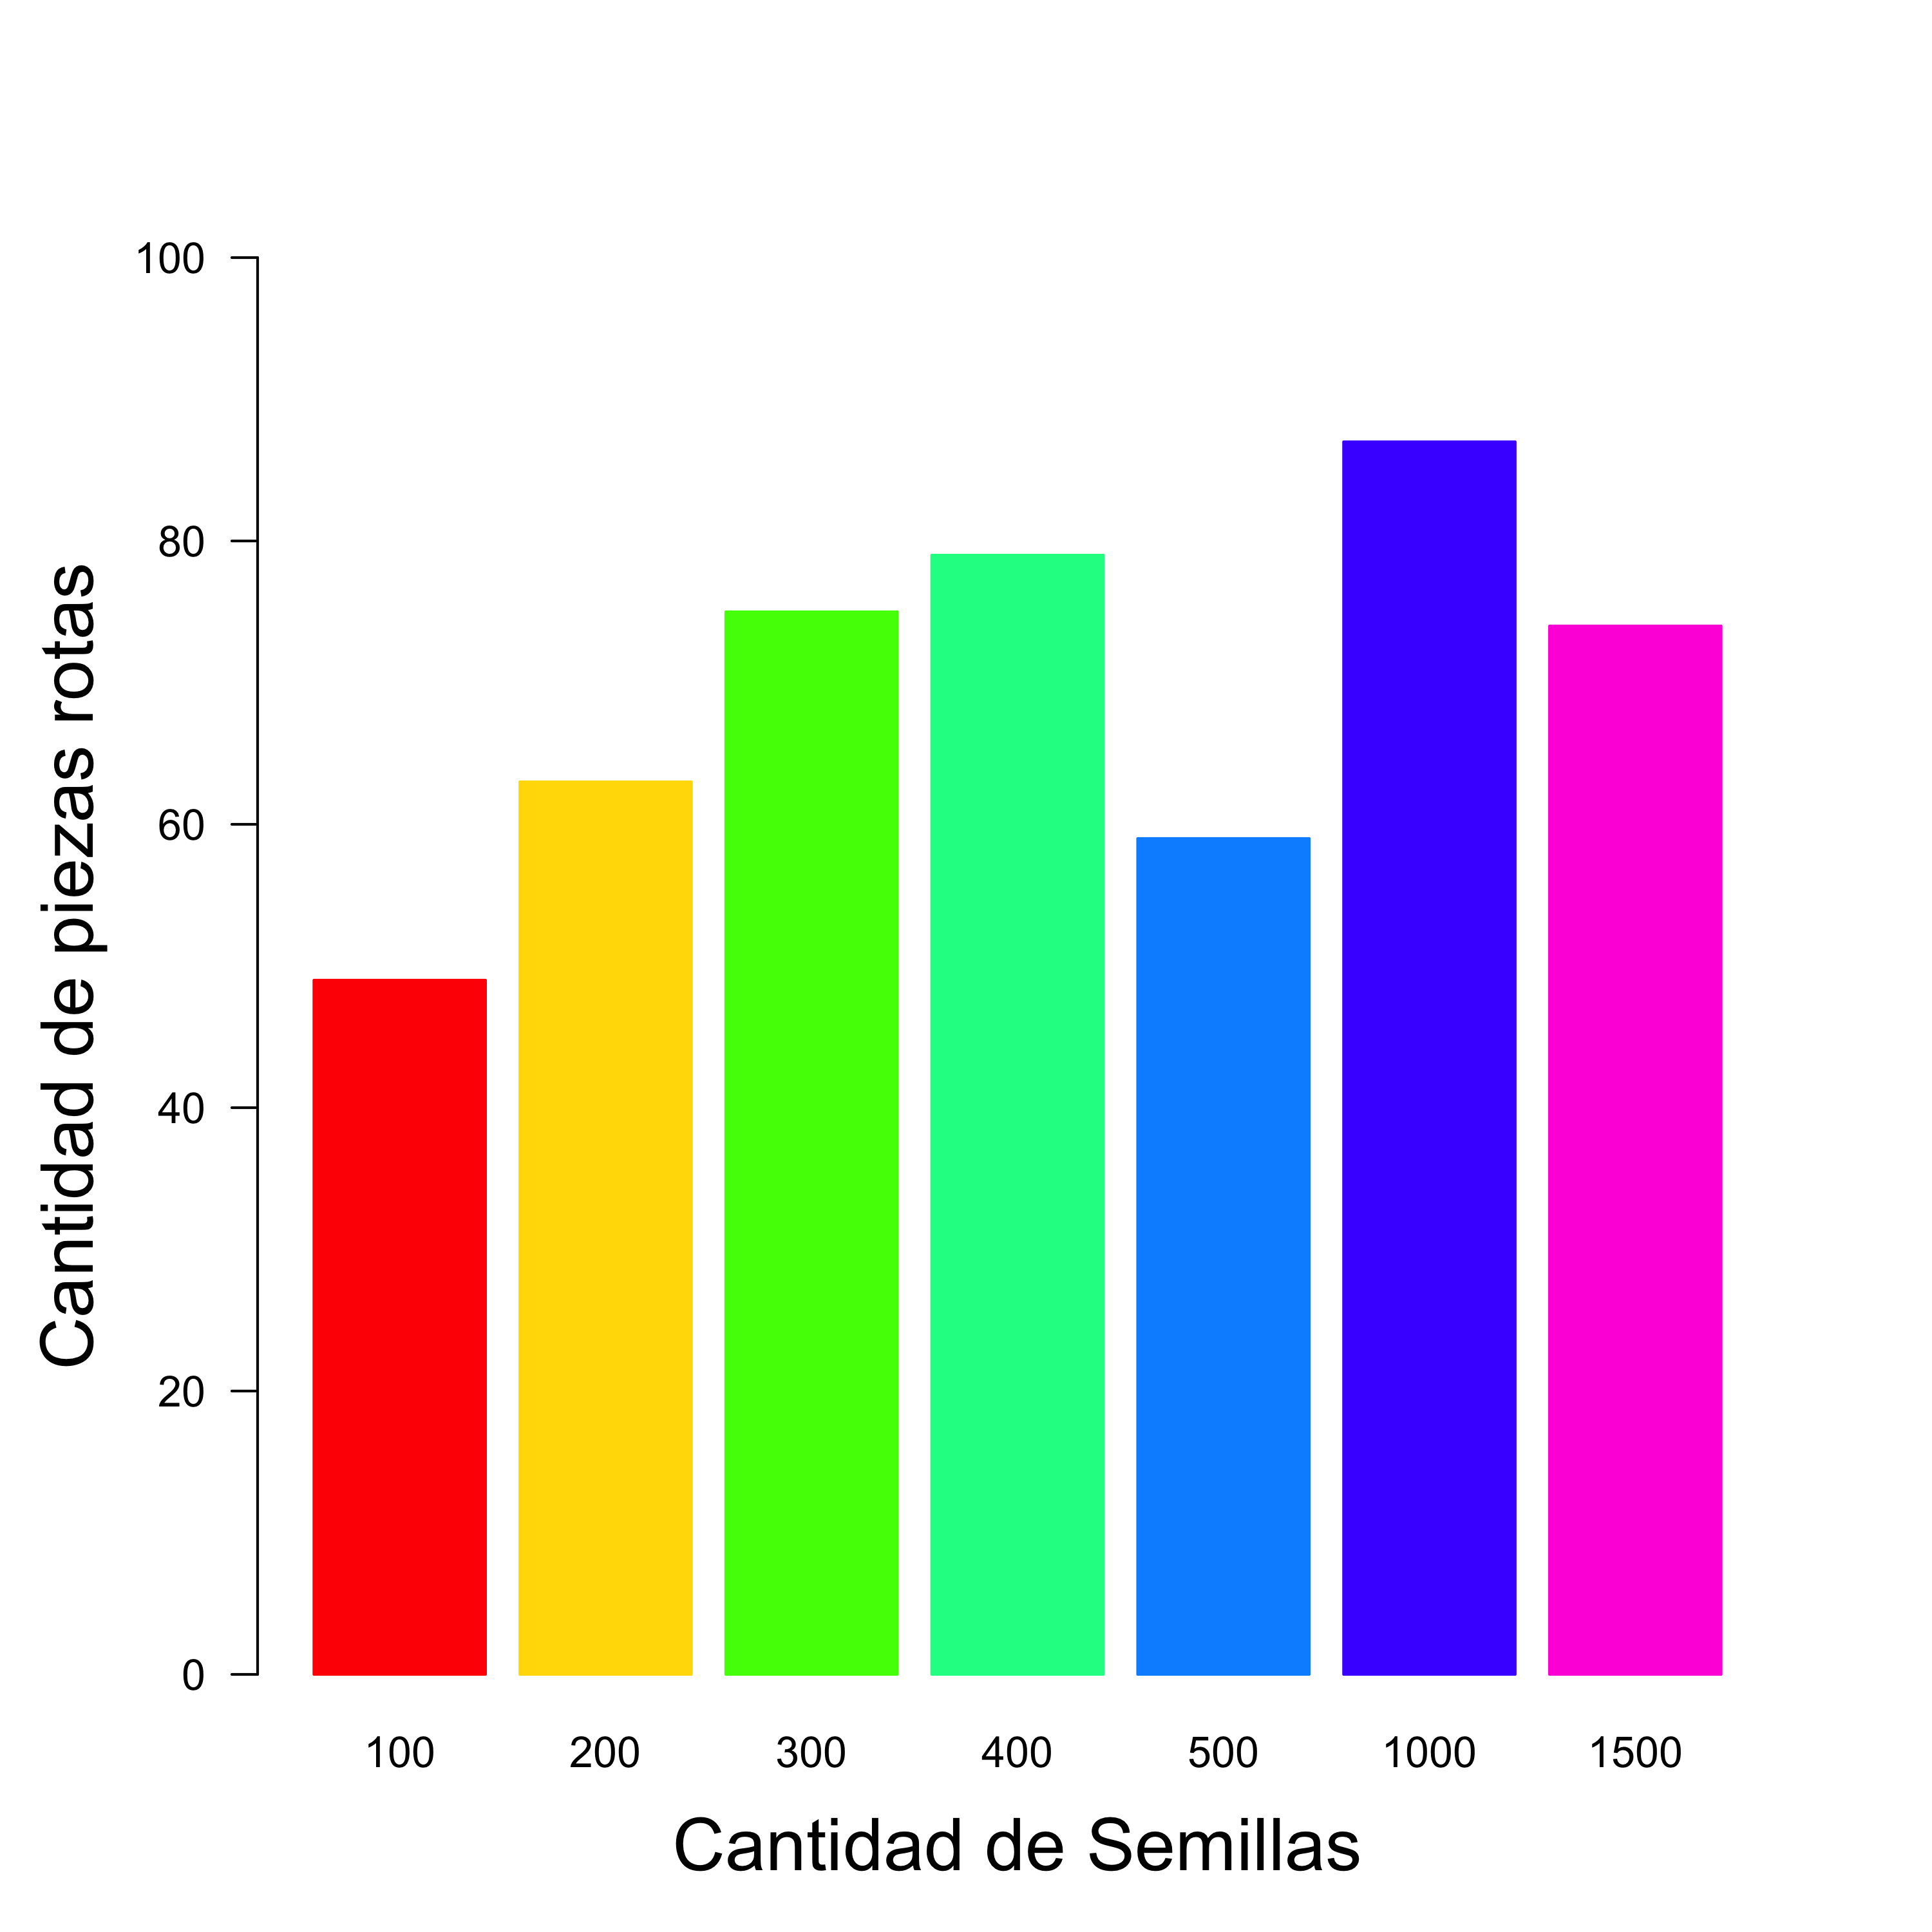
\includegraphics[width=\linewidth]{50.png}
 		 \caption{Tamaño $50\times 50$.}
 		\label{b50}
 	\end{subfigure}
 	\begin{subfigure}[b]{0.3\linewidth}
 		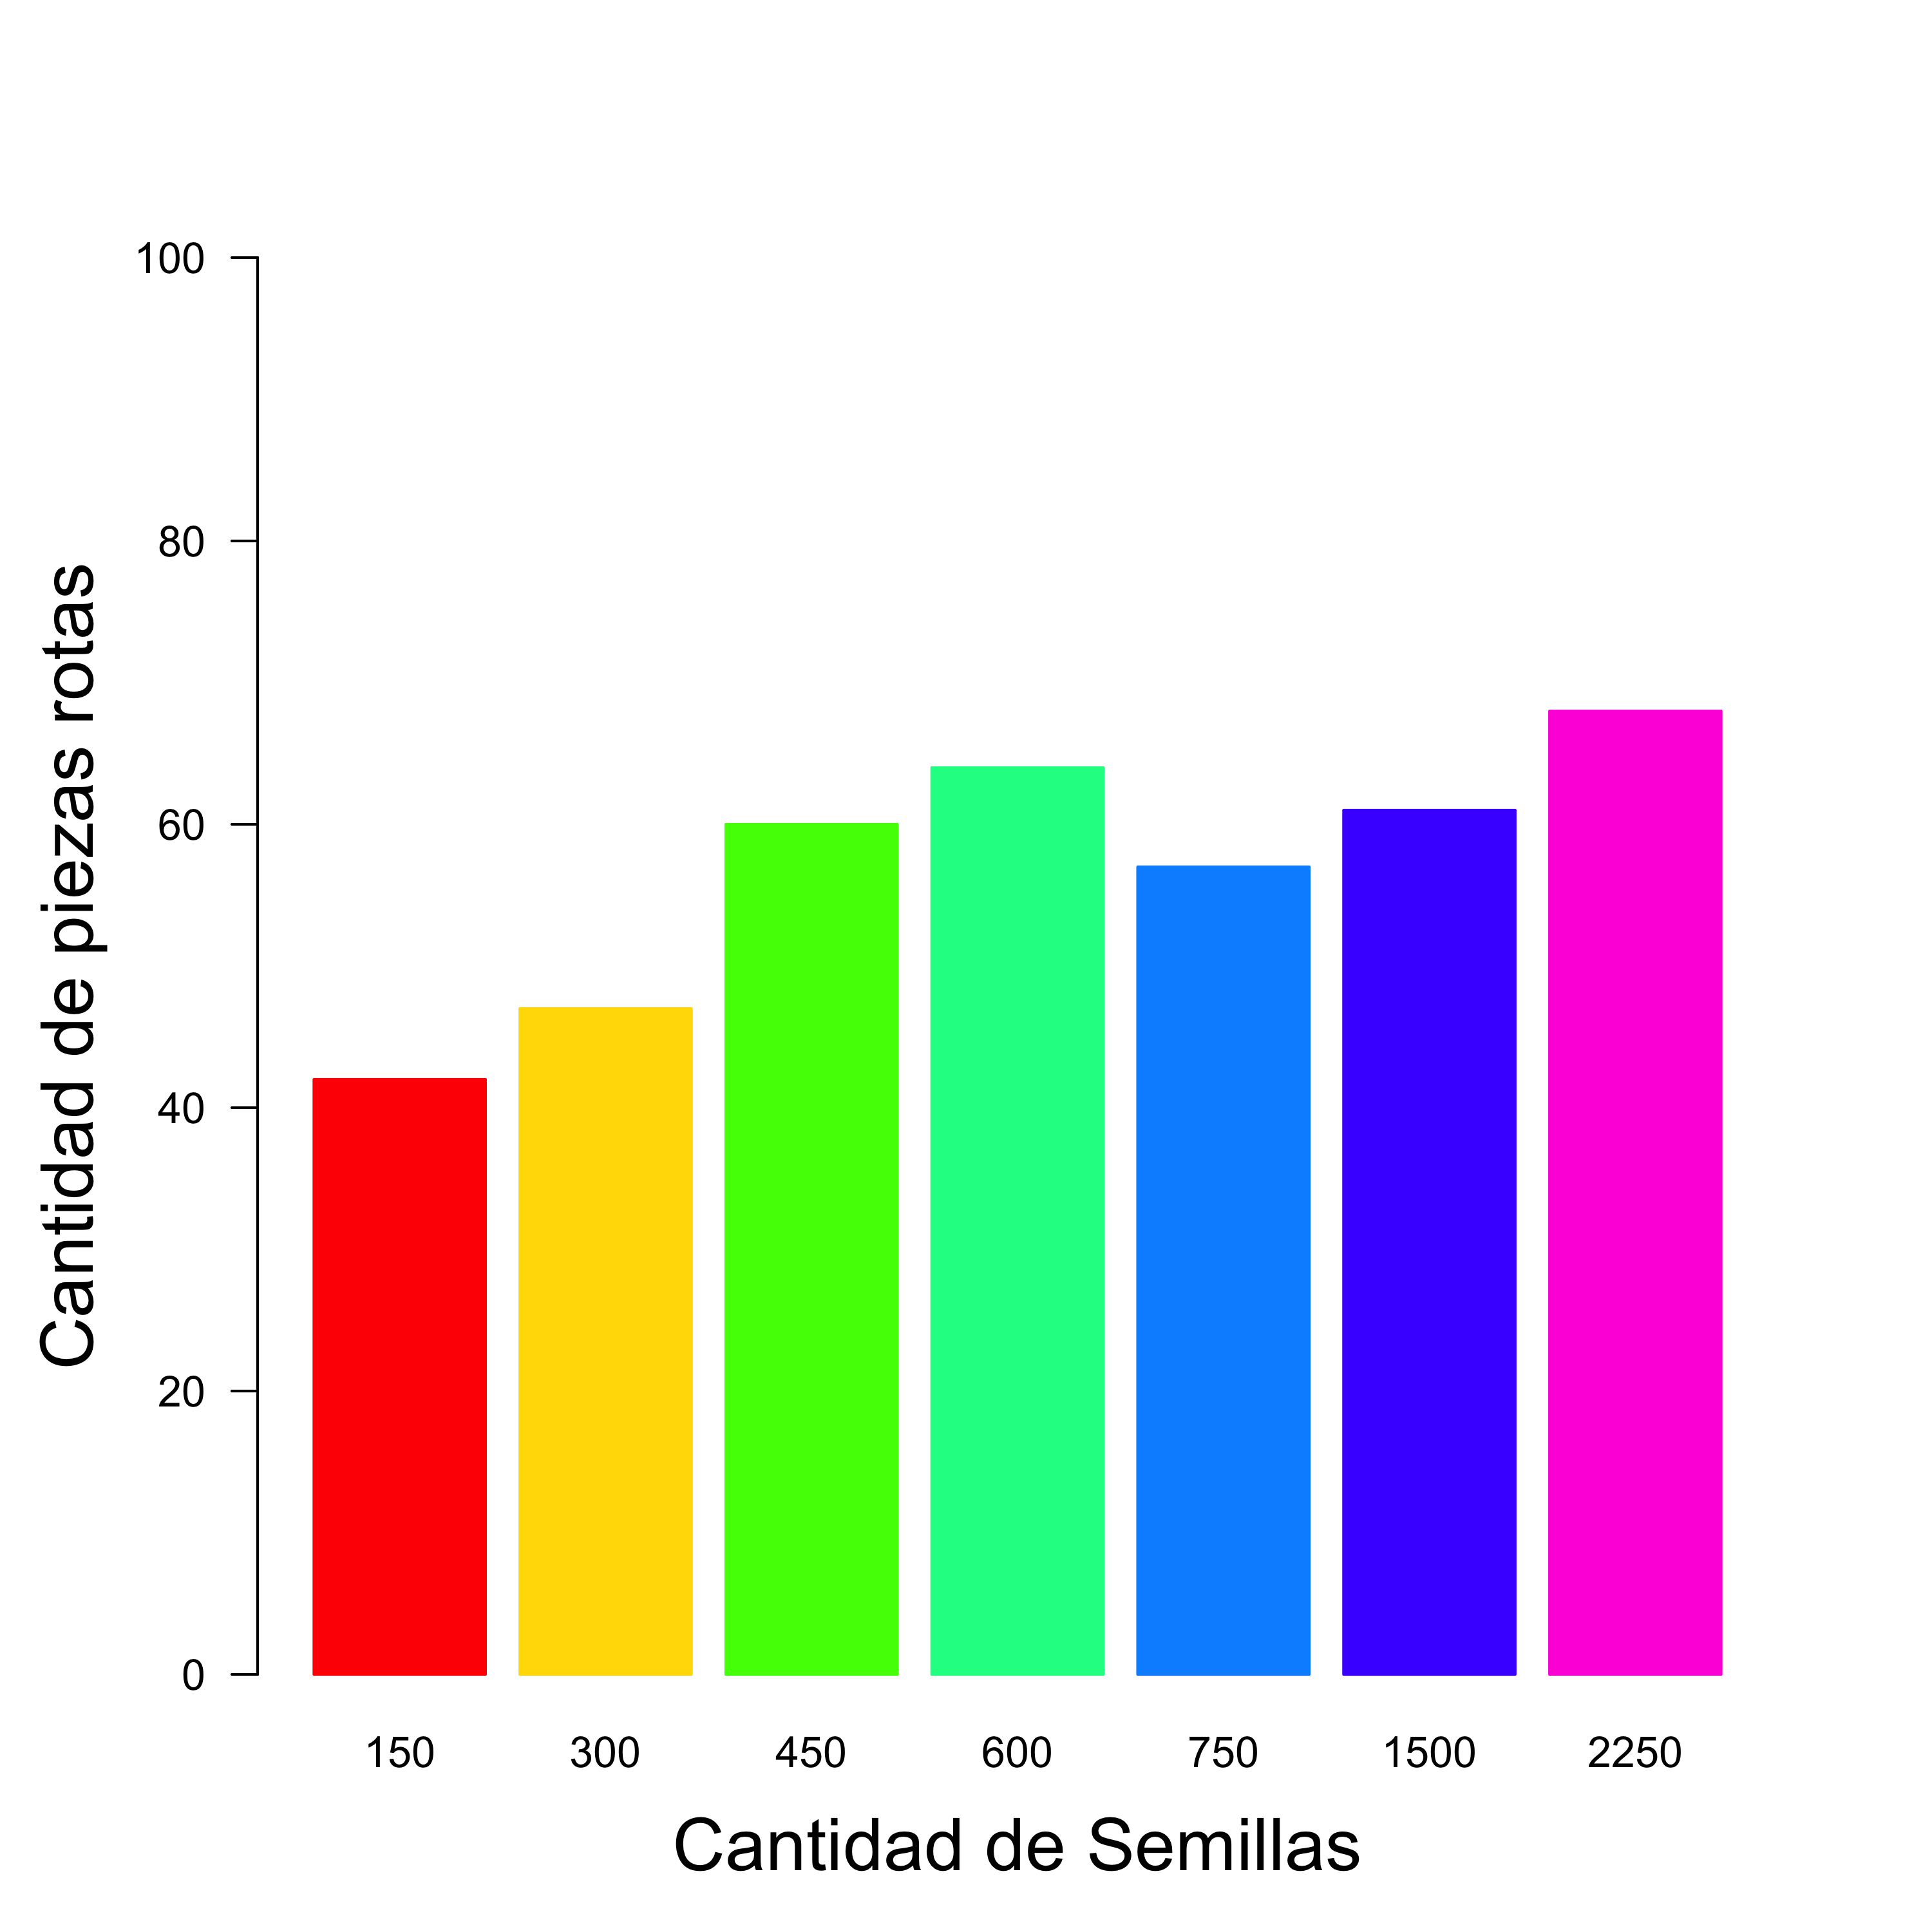
\includegraphics[width=\linewidth]{75.png}
 		 \caption{Tamaño $75\times 75$.}
 		\label{b75}
 	\end{subfigure}
 	\begin{subfigure}[b]{0.3\linewidth}
 		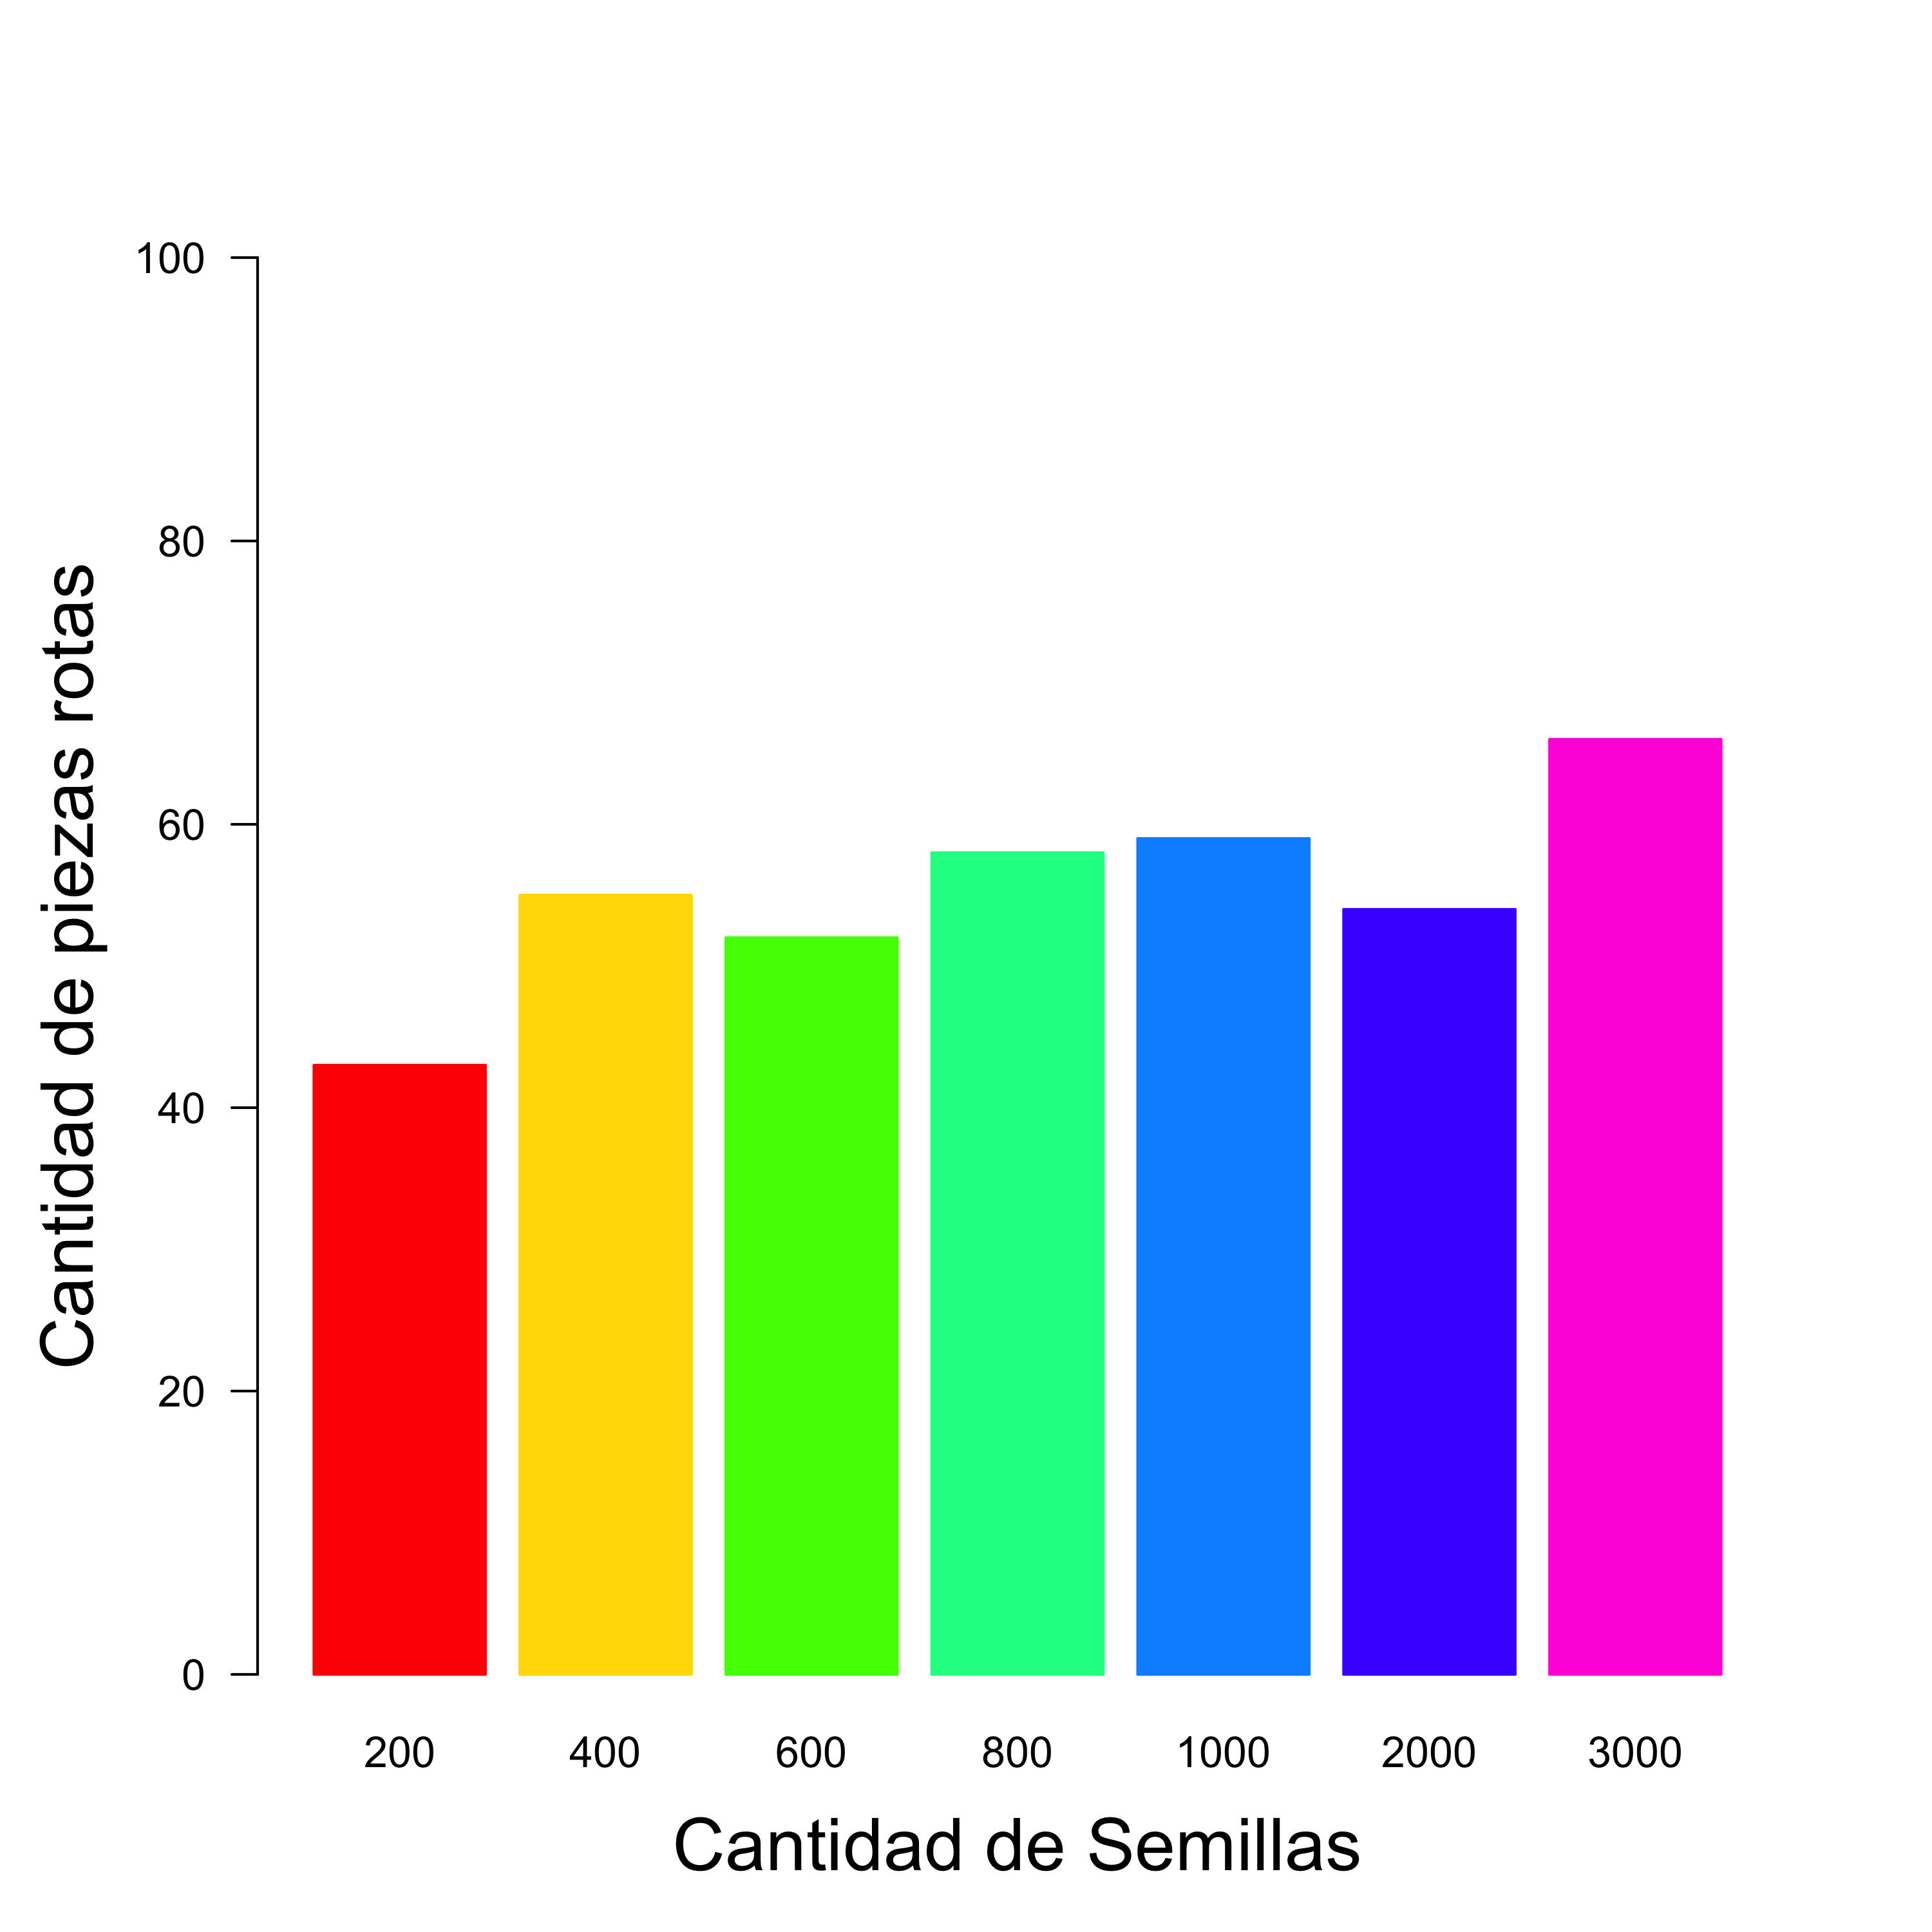
\includegraphics[width=\linewidth]{100.png}
 		\caption{Tamaño $100 \times 100$.}
 		\label{b100}
 	\end{subfigure}
 	 	\begin{subfigure}[b]{0.3\linewidth}
 		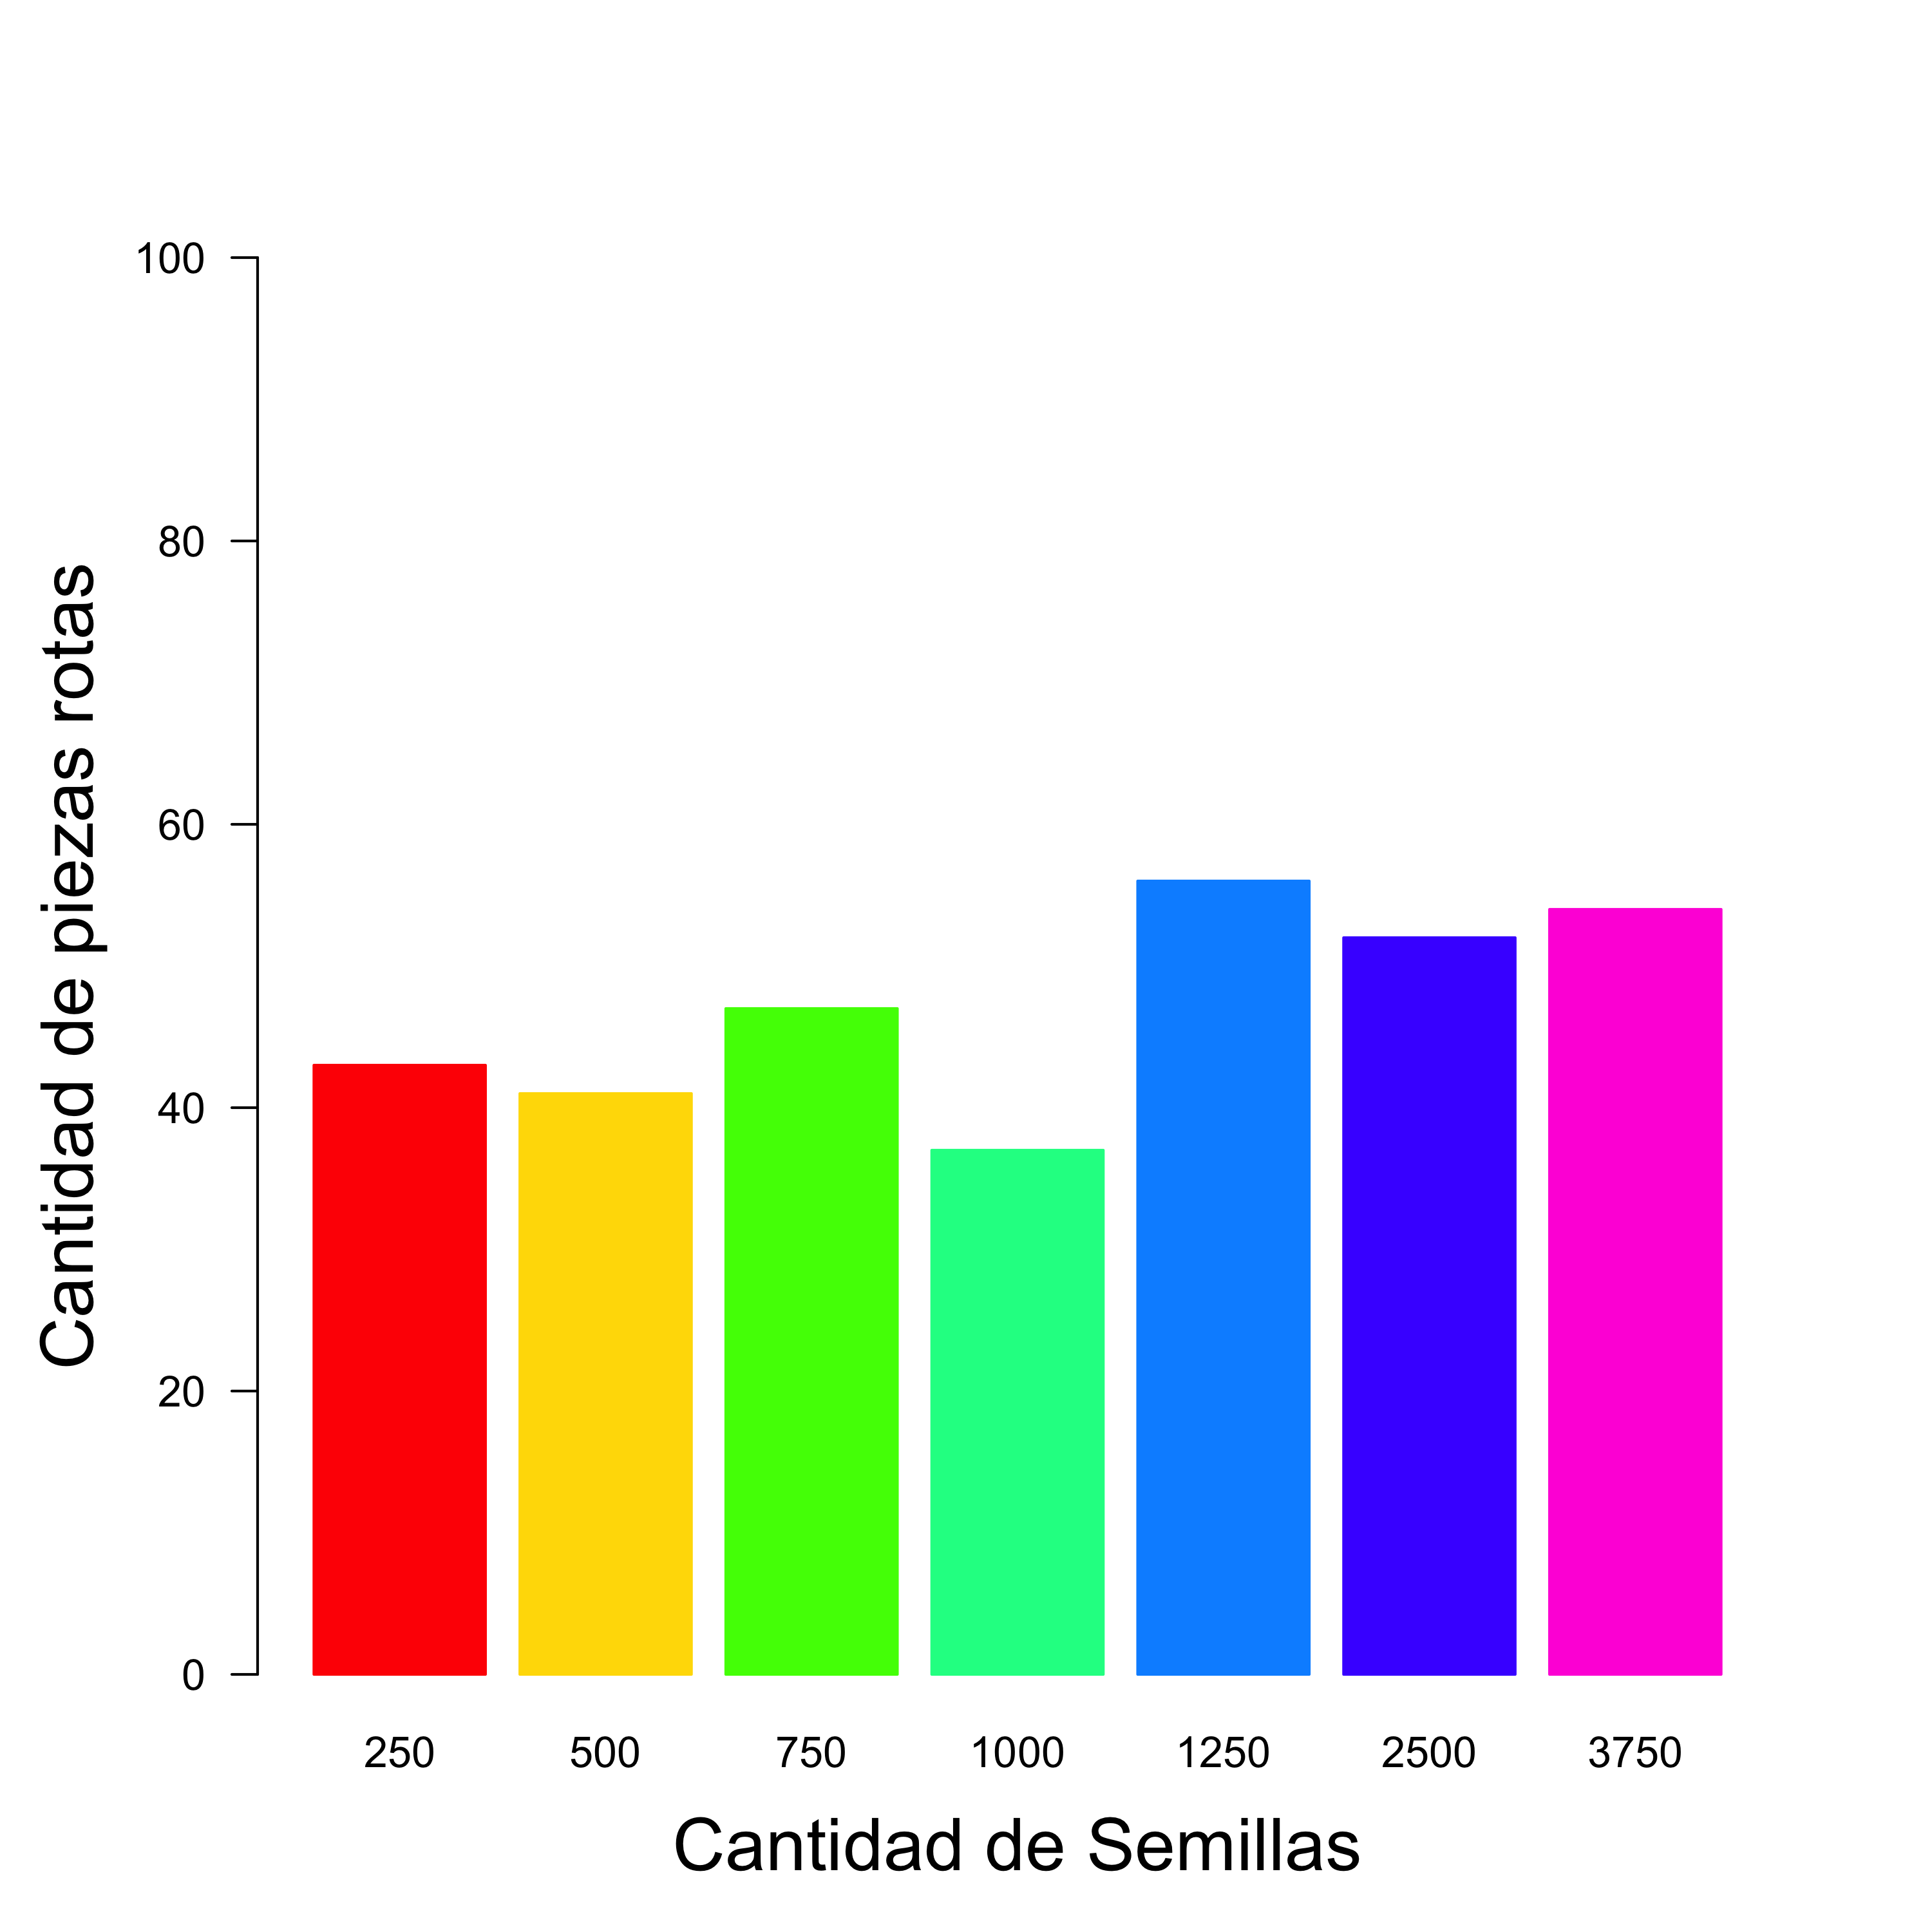
\includegraphics[width=\linewidth]{125.png}
 		 \caption{Tamaño $125 \times 125$.}
 		\label{b125}
 	\end{subfigure}
 	\begin{subfigure}[b]{0.3\linewidth}
 		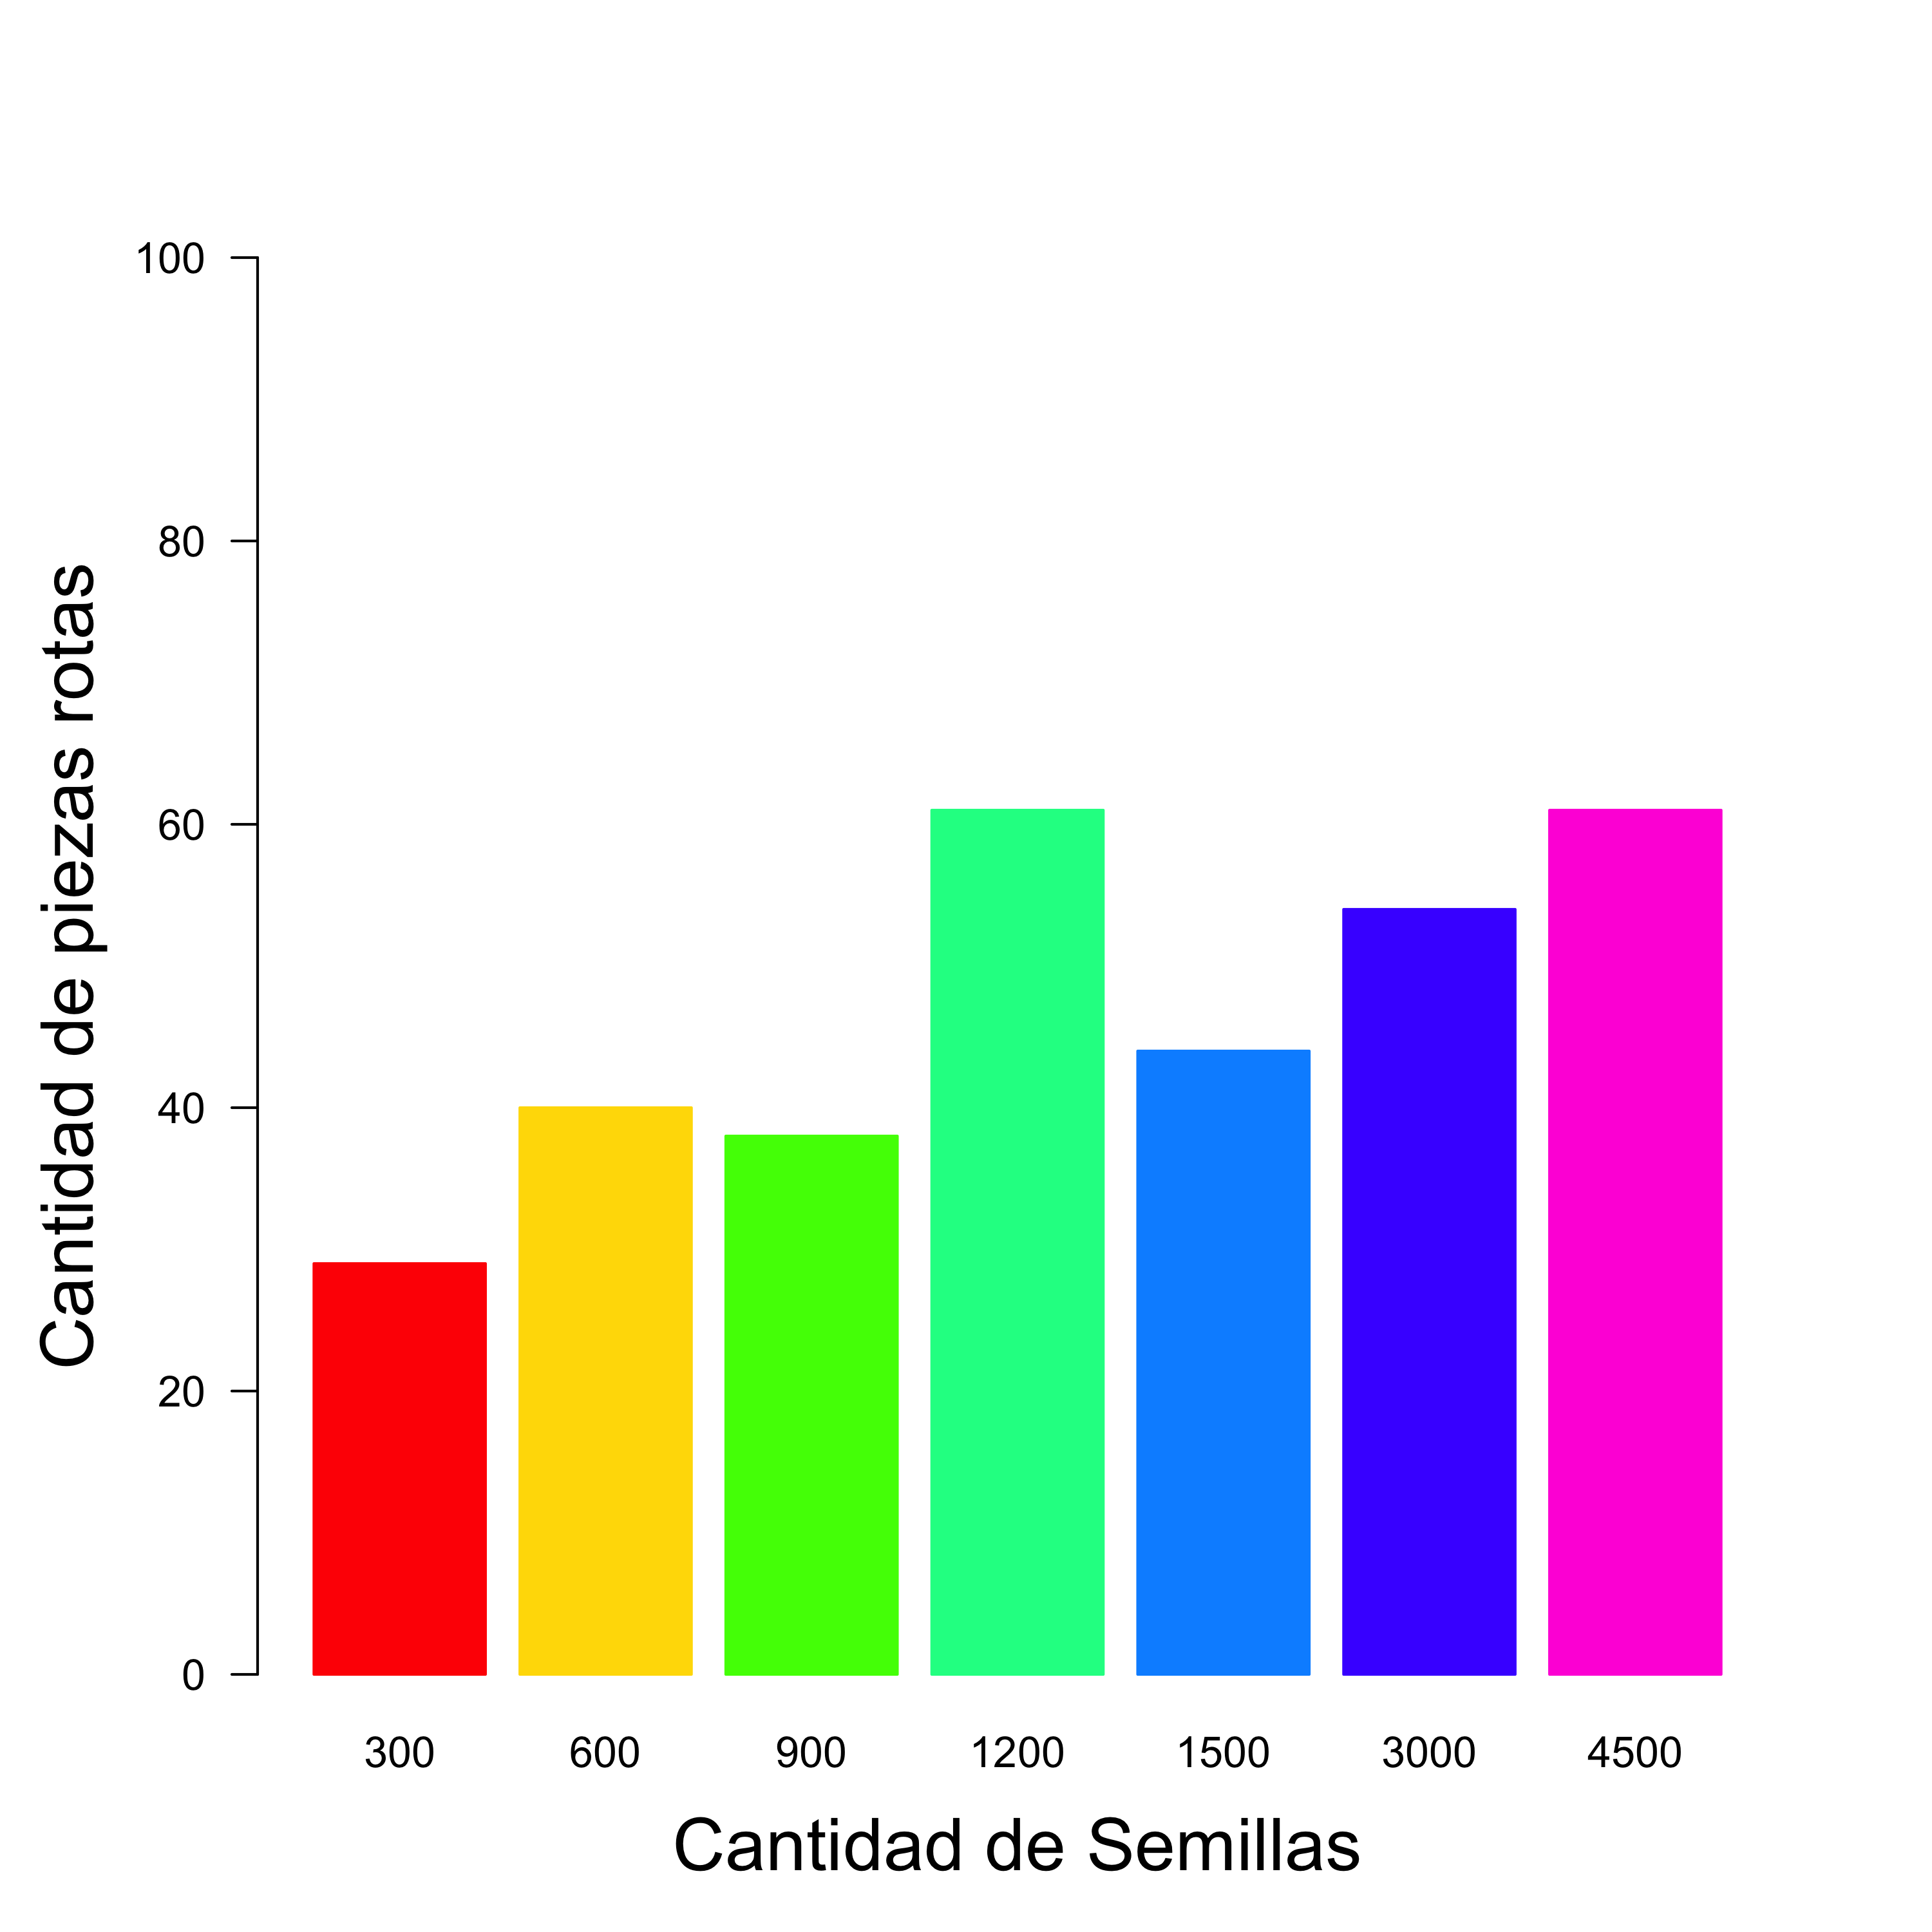
\includegraphics[width=\linewidth]{150.png}
 		 \caption{Tamaño $150 \times 150$.}
 		\label{b150}
 	\end{subfigure}
 	\begin{subfigure}[b]{0.3\linewidth}
 		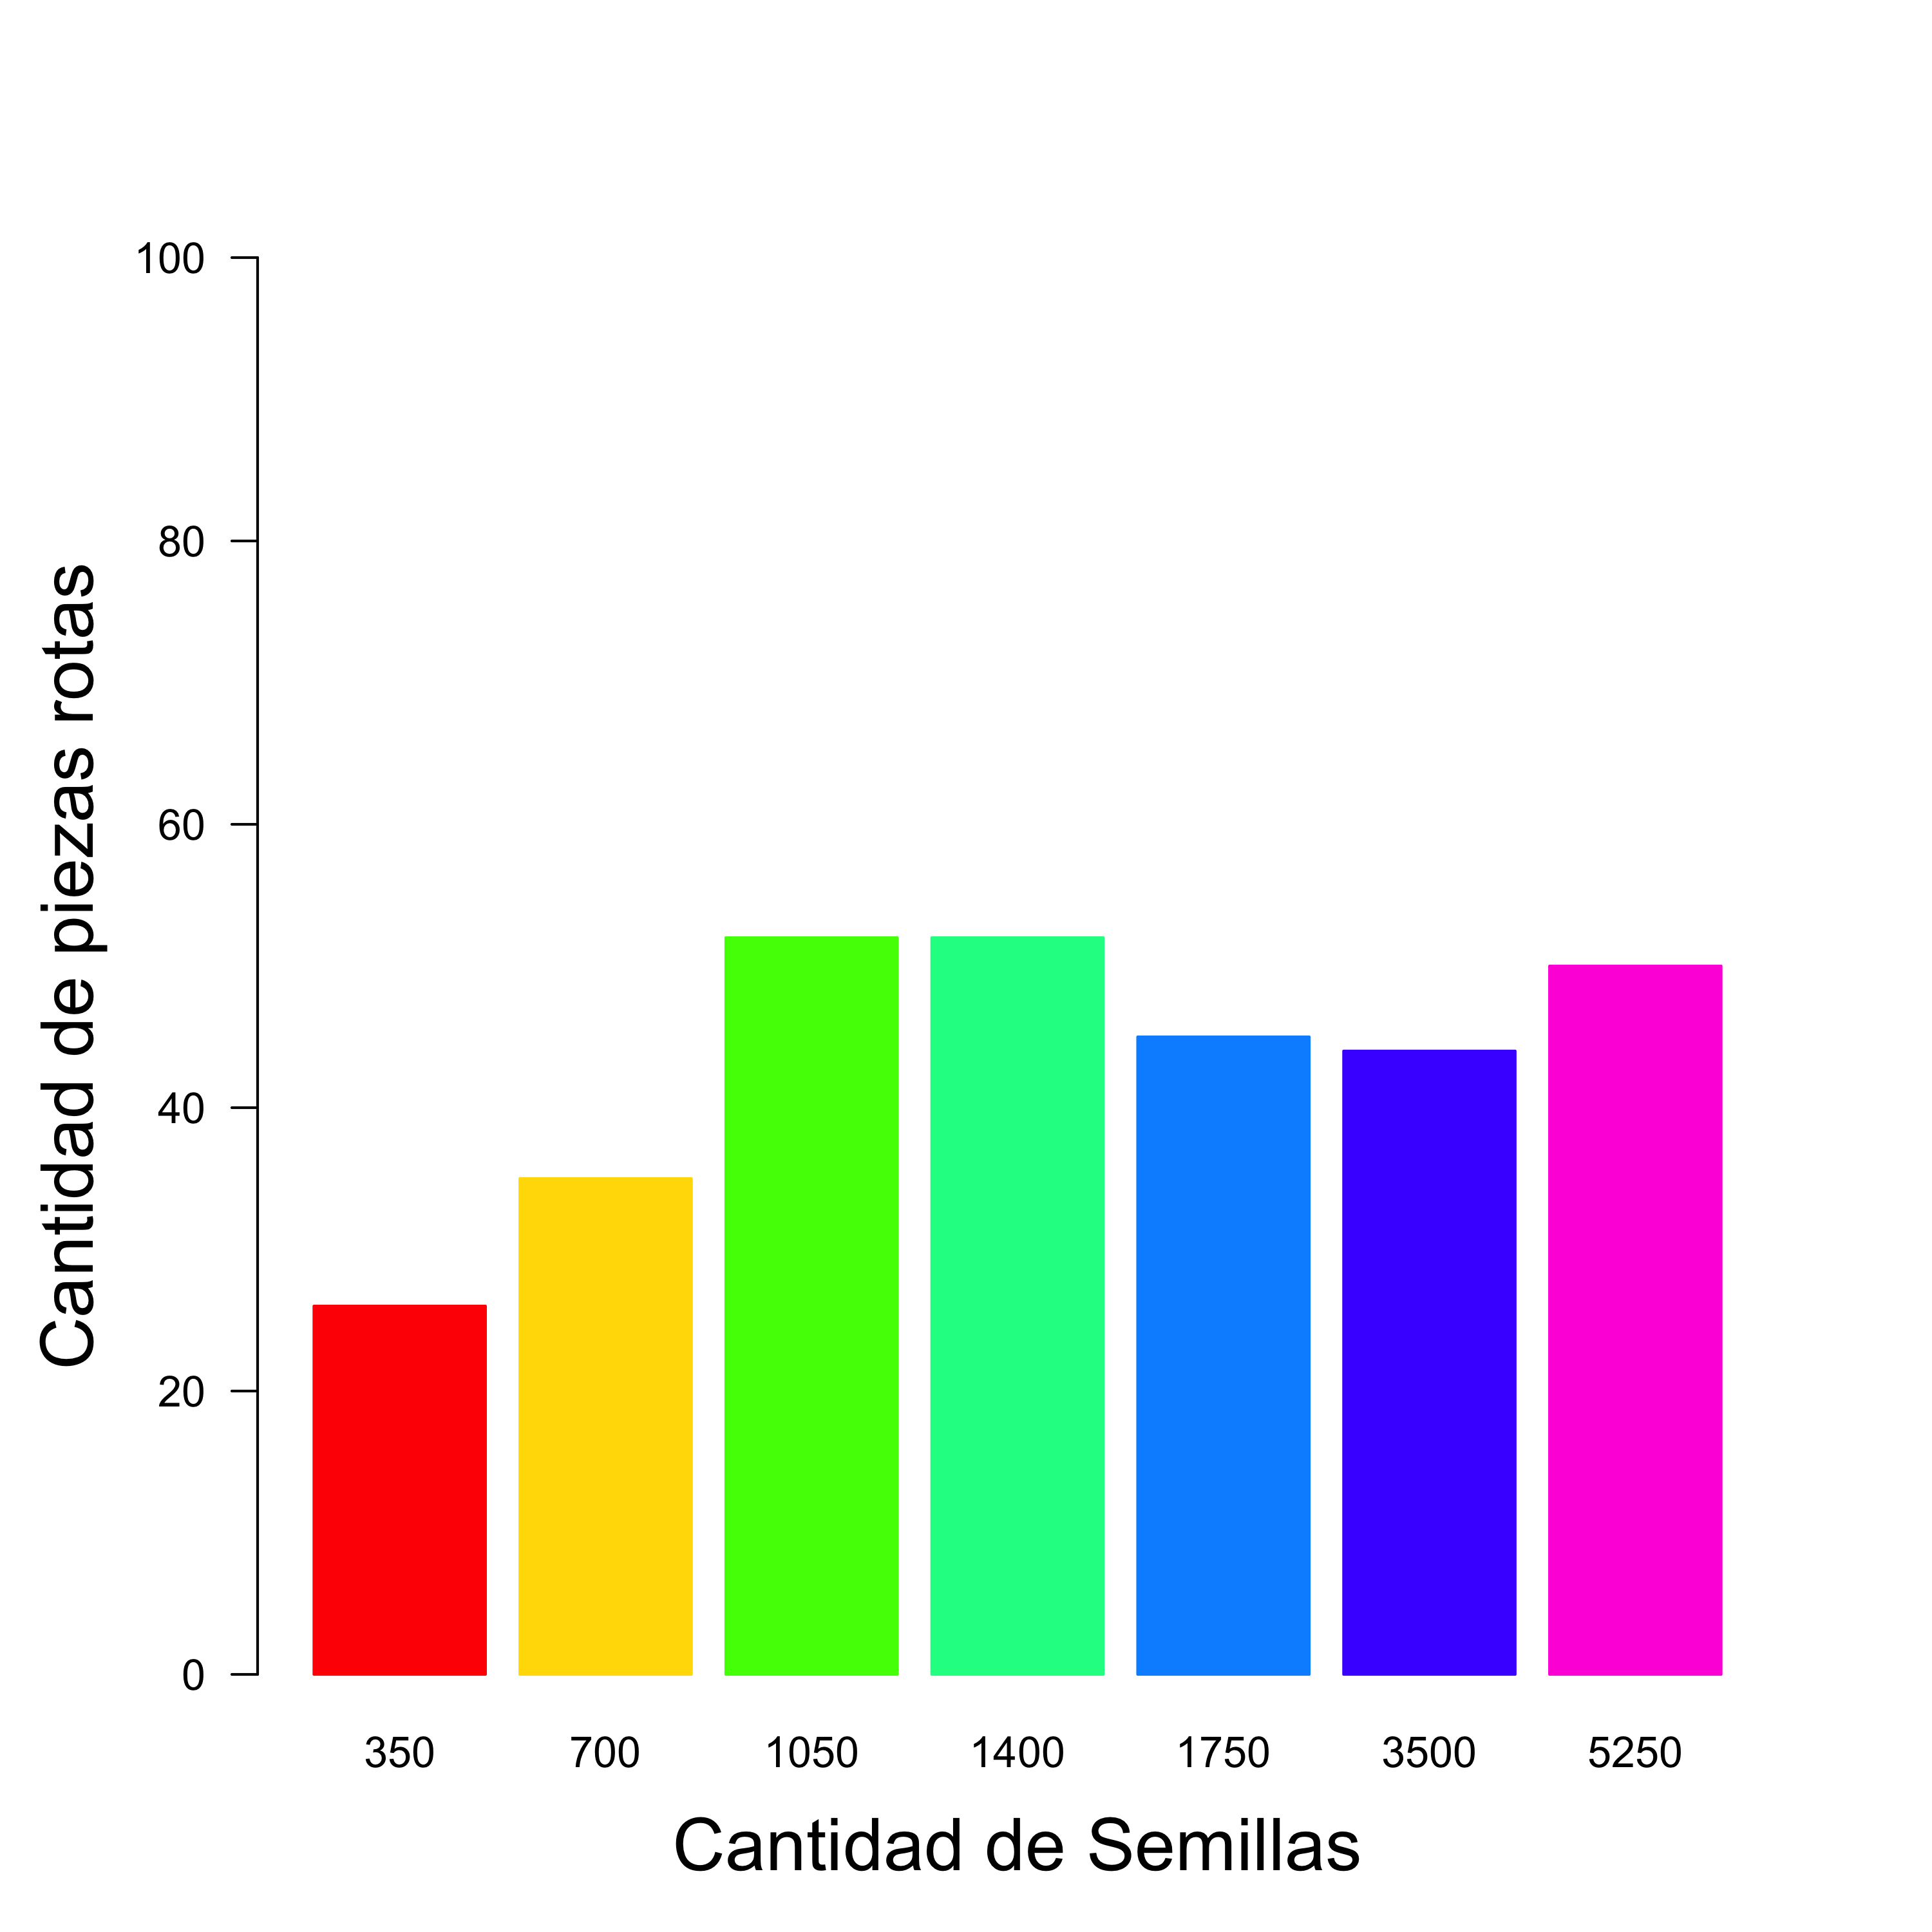
\includegraphics[width=\linewidth]{175.png}
 		\caption{Tamaño $175 \times 175$.}
 		\label{b175}
 	\end{subfigure}
 	 	\begin{subfigure}[b]{0.3\linewidth}
 		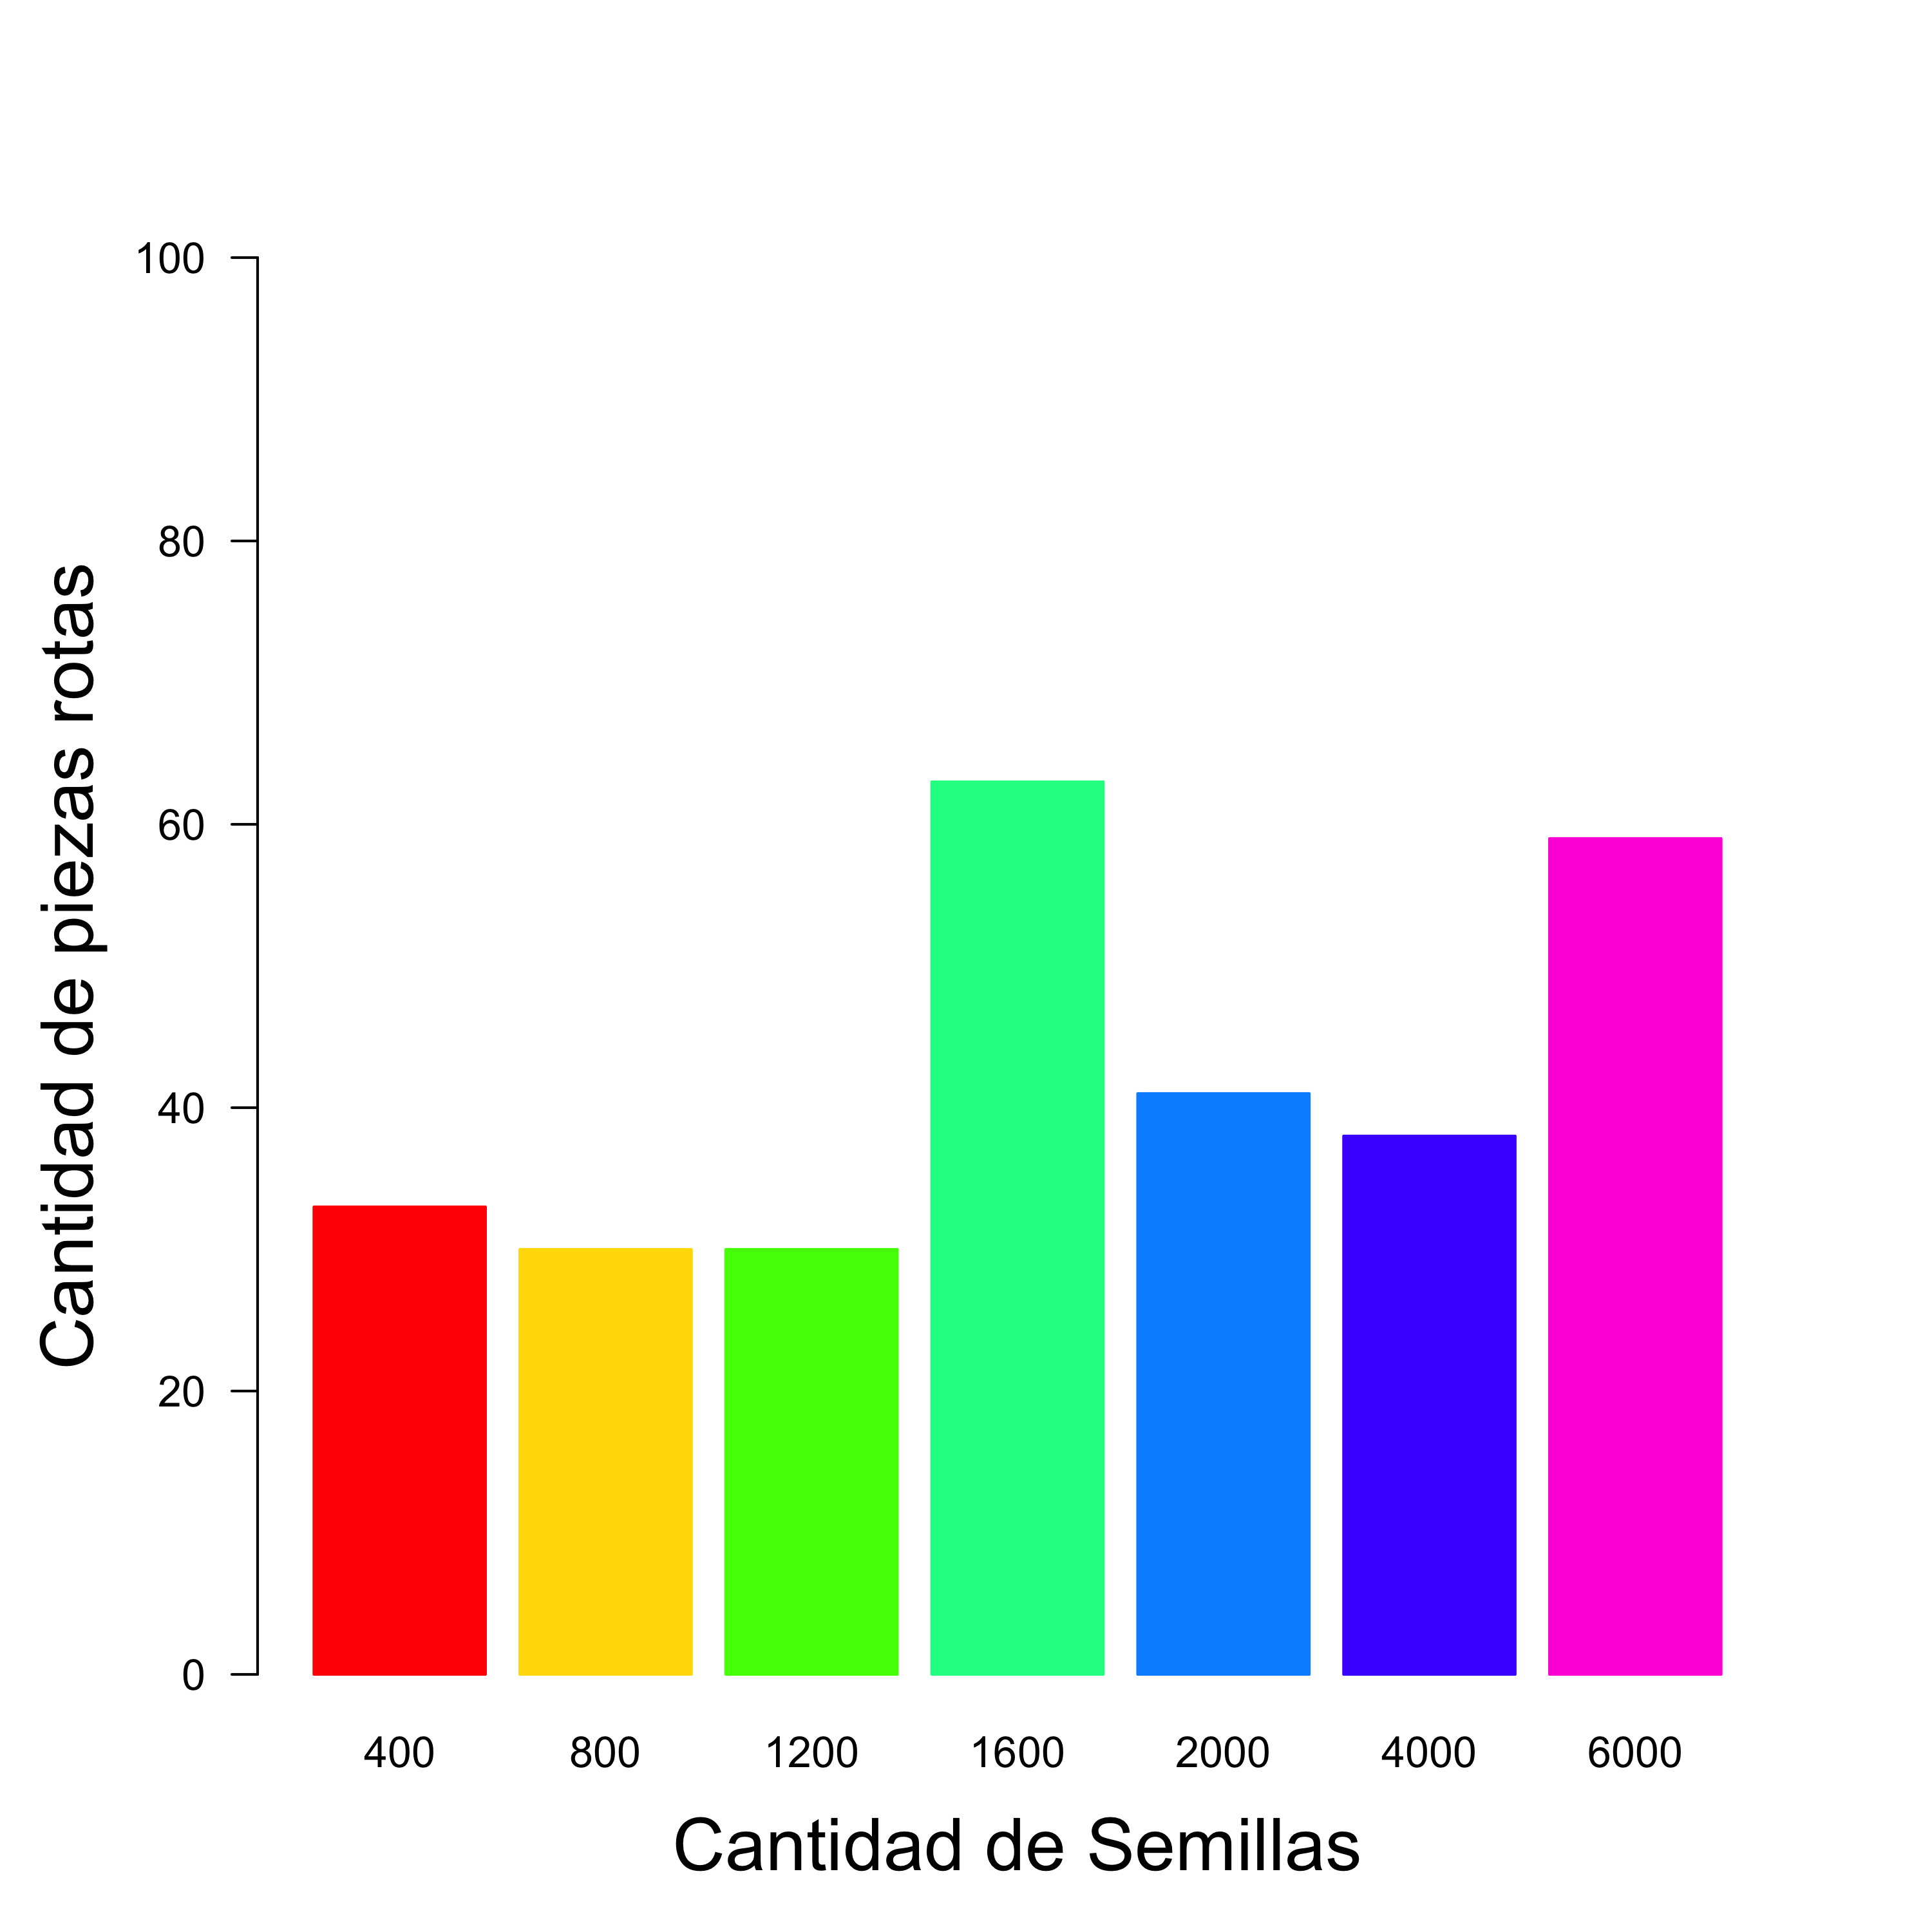
\includegraphics[width=\linewidth]{200.png}
 		\caption{Tamaño $200 \times 200$.}
 		\label{b200}
 	\end{subfigure}
 	\caption{Gráfica de barras de las piezas rotas variando el tamaño de la pieza y cantidad de semillas.}  		
\label{barplot}
 \end{figure}
 
 \begin{figure}
 	\centering
 	\begin{subfigure}[b]{0.28\linewidth}
 		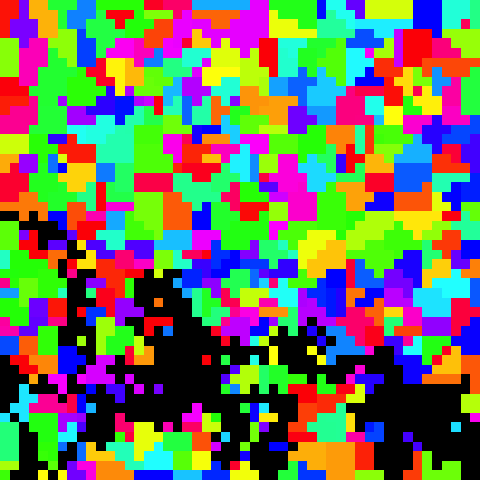
\includegraphics[width=\linewidth]{p4g_63.png}
 		 \caption{}
 		\label{grieta1}
 	\end{subfigure}
 	\begin{subfigure}[b]{0.28\linewidth}
 		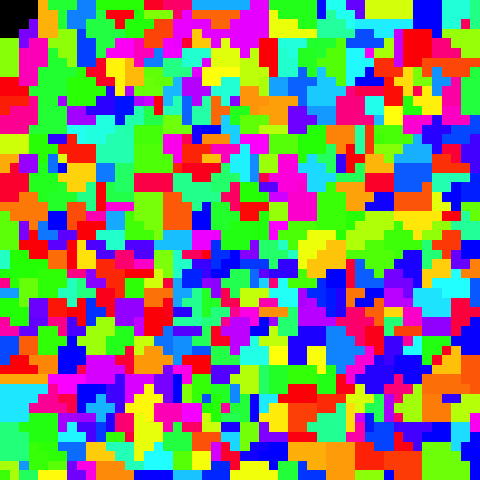
\includegraphics[width=\linewidth]{p4g_37.png}
 		 \caption{}
 		\label{grieta2}
 	\end{subfigure}
 	\begin{subfigure}[b]{0.28\linewidth}
 		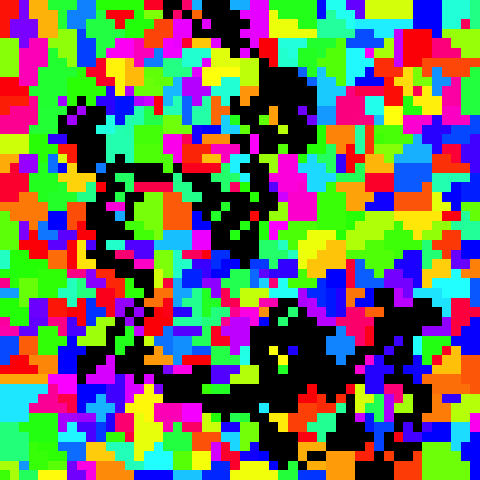
\includegraphics[width=\linewidth]{p4g_187.png}
 		\caption{}
 		\label{grieta3}
 	\end{subfigure}
 	\caption{Ejemplos de grietas en una pieza de 50 $\times$ 50.}  	
\label{grieta}
 \end{figure}

\subsection{Pruebas de correlación}
Se realiza una prueba para verificar si existe correlación entre los datos de las columnas del cuadro \ref{datos}. Para ello se utiliza la función \texttt{cor.test}. Primeramente, aplicamos la prueba para ver si hay, o no, correlación entre la cantidad de semillas y la cantidad de piezas rotas, obteniendo un valor $p$ de 0.5446, por lo que se concluye que no hay correlación. Es decir, la cantidad de semillas no afecta a la cantidad de piezas rotas.

\begin{verbatim}
Pearson's product-moment correlation

data:  datos$Semilla and datos$Cantidad de piezas rotas
t = 0.61036, df = 47, p-value = 0.5446
alternative hypothesis: true correlation is not equal to 0
95 percent confidence interval:
 -0.1974405  0.3608772
sample estimates:
       cor 
0.08867956 
\end{verbatim}

Ahora, se realiza la prueba de correlación para las columnas del tamaño y cantidad de piezas rotas. La prueba arroja un valor $p$ de $2.44\times 10^{-8}$ el cual es menor que 0.05, por lo que se rechaza la hipótesis nula y se concluye que hay correlación entre estas variables. Es decir, el tamaño de la pieza afecta a la cantidad de piezas rotas. En particular, se estima el coeficiente de correlación en -0.699, por lo que se concluye que a mayor tamaño de la pieza, menos piezas se rompen.

\begin{verbatim}
Pearson's product-moment correlation

data:  datos$Tamaño and datos$Cantidad de piezas rotas
t = -6.7111, df = 47, p-value = 2.244e-08
alternative hypothesis: true correlation is not equal to 0
95 percent confidence interval:
 -0.8195231 -0.5207744
sample estimates:
       cor 
-0.6995316 
\end{verbatim}

\bibliographystyle{plain} 
\bibliography{Referencias}


\end{document} 